\documentclass{article}

\usepackage{amsmath}
\usepackage{amsthm}
\usepackage{amssymb}
\usepackage{bbm}
\usepackage{fancyhdr}
% \usepackage{listings}
\usepackage{cite}
\usepackage{graphicx}
\usepackage{enumitem}
\usepackage{courier}
\usepackage[pdftex,colorlinks=true, urlcolor = blue]{hyperref}


\oddsidemargin 0in \evensidemargin 0in
\topmargin -0.5in \headheight 0.25in \headsep 0.25in
\textwidth 6.5in \textheight 9in
\parskip 6pt \parindent 0in \footskip 20pt

% set the header up
\fancyhead{}
\fancyhead[L]{Stanford Aeronautics \& Astronautics}
\fancyhead[R]{Fall 2020}

%%%%%%%%%%%%%%%%%%%%%%%%%%
\renewcommand\headrulewidth{0.4pt}
\setlength\headheight{15pt}

\usepackage{xparse}
\NewDocumentCommand{\codeword}{v}{%
\texttt{\textcolor{blue}{#1}}%
}

\usepackage{xcolor}
\setlength{\parindent}{0in}

\title{AA 274A: Principles of Robot Autonomy I \\ Problem Set X}
\author{Name: Li Quan Khoo (SCPD)     \\ SUID: lqkhoo}
\date{}

\begin{document}

\maketitle
\pagestyle{fancy} 

\section*{Problem 1: Trajectory Generation via Differential Flatness}
\begin{enumerate}[label=(\roman*)]
\item % (i)

We are given initial and final conditions in terms of variables $\{x, y, V, \theta\}$. The equations are:

$$
\begin{bmatrix}
1 & 0   & 0      & 0 \\
0 & 1   & 0      & 0 \\
1 & t_f & t_f^2  & t_f^3 \\
0 & 1   & 2 t_f  & 3 t_f^2
\end{bmatrix}
\begin{bmatrix}
x_1 \\ x_2 \\ x_3 \\ x_4
\end{bmatrix}
=
\begin{bmatrix}
x(0) \\ \dot{x}(0) \\ x(t_f) \\ \dot{x}(t_f)
\end{bmatrix}
$$

$$
\begin{bmatrix}
1 & 0   & 0      & 0 \\
0 & 1   & 0      & 0 \\
1 & t_f & t_f^2  & t_f^3 \\
0 & 1   & 2 t_f  & 3 t_f^2
\end{bmatrix}
\begin{bmatrix}
y_1 \\ y_2 \\ y_3 \\ y_4
\end{bmatrix}
=
\begin{bmatrix}
y(0) \\ \dot{y}(0) \\ y(t_f) \\ \dot{y}(t_f)
\end{bmatrix}
$$

where $\dot{x}(t)=V\cos\theta$ and $\dot{y}(t)=V\sin\theta$ as given by the robot's kinematic model.


\item % (ii)
Since $\det(J)=V$, $V>0\; \forall t$ is a sufficient and necessary condition for the matrix $J$ to be invertible.

\item % (iii)
(code)

\item % (iv)
(code)

\item % (v)
\begin{tabular}[t]{c}
	\hline \\
	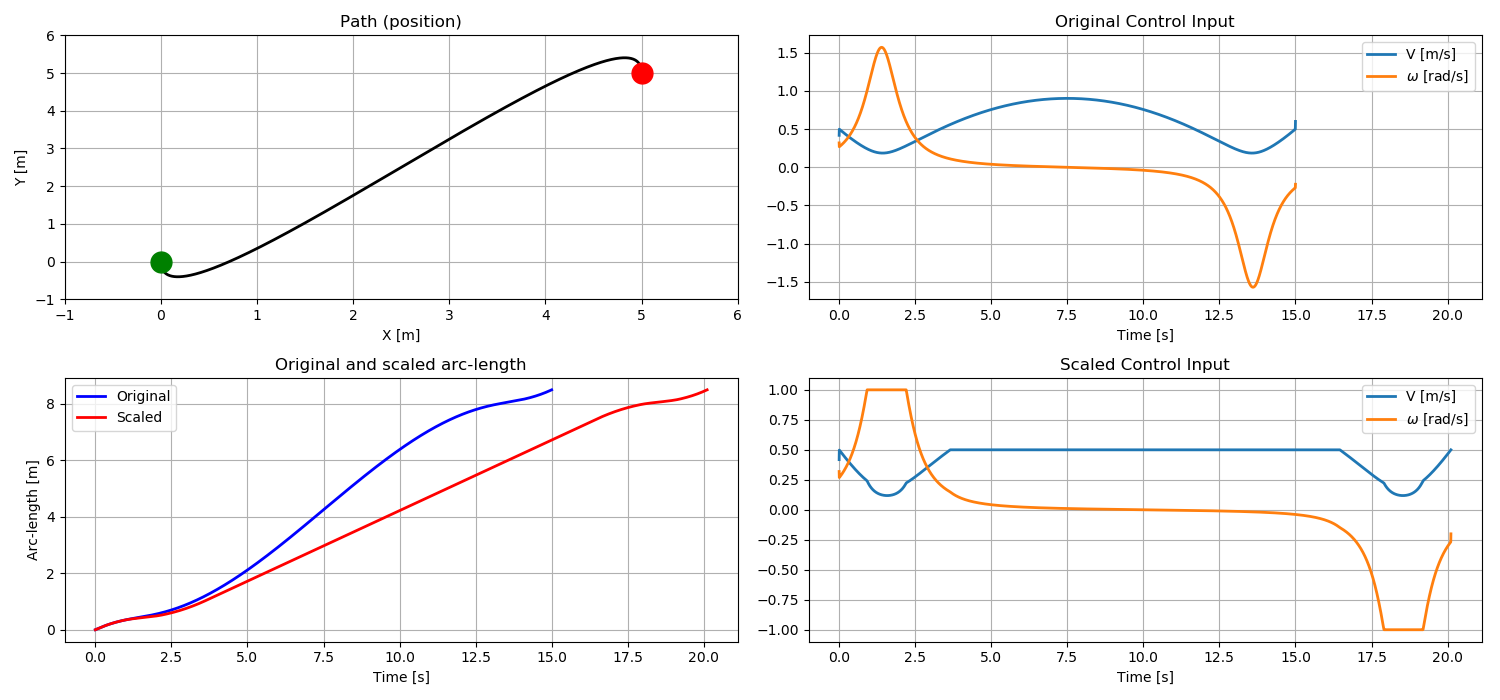
\includegraphics[width=1.0\textwidth]{img/differential_flatness.png} \\
	Trajectory of unicycle model in absence of noise. Initial and final conditions as given. \\
	\hline
\end{tabular}

\item % (vi)
\begin{tabular}[t]{c}
	\hline \\
	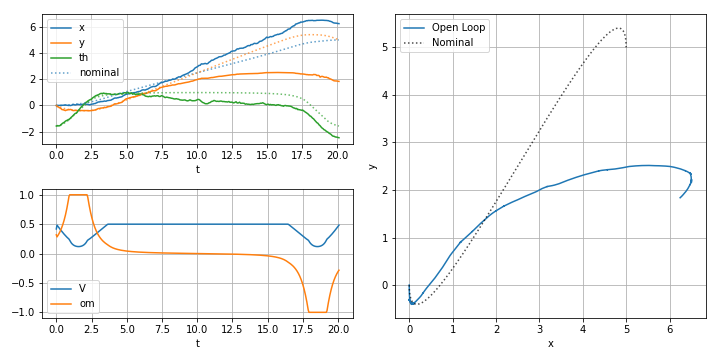
\includegraphics[width=1.0\textwidth]{img/sim_traj_openloop.png} \\
	Trajectory of unicycle model where control vector $u_\text{noisy}=u + \epsilon$ where $\epsilon$ is simulated isotropic Gaussian noise. \\
	\hline
\end{tabular}


\end{enumerate}

\section*{Problem 2: Pose Stabilization}

	\begin{enumerate}[label=(\roman*)]
		
	\item % (i)
	(code)
	
	\item % (ii)
	(code)
	
	\item % (iii)
	\begin{tabular}[t]{c}
		\hline \\
		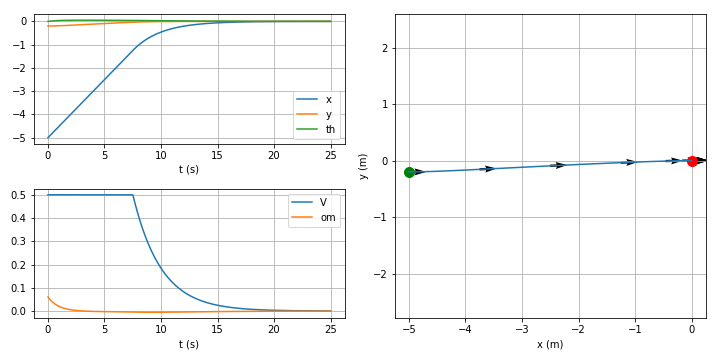
\includegraphics[width=1.0\textwidth]{img/sim_parking_forward.png} \\
		Forward parking \\
		\hline
	\end{tabular}
	\begin{tabular}[t]{c}
		\hline \\
		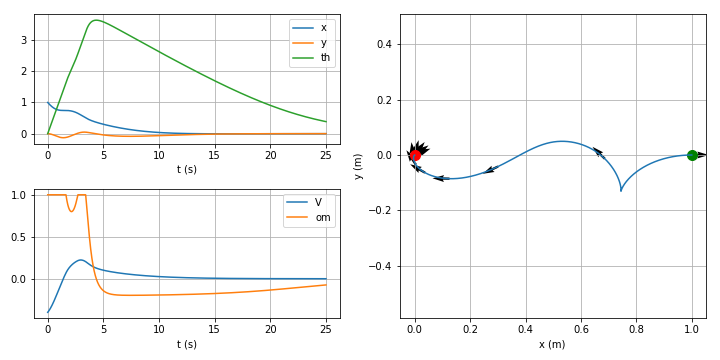
\includegraphics[width=1.0\textwidth]{img/sim_parking_reverse.png} \\
		Reverse parking \\
		\hline
	\end{tabular}
	\begin{tabular}[t]{c}
		\hline \\
		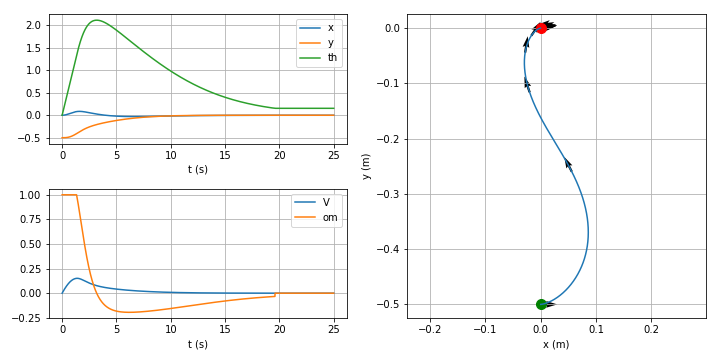
\includegraphics[width=1.0\textwidth]{img/sim_parking_parallel.png} \\
		Parallel parking \\
		\hline
	\end{tabular}
		
	\end{enumerate}


\section*{Problem 3: Trajectory Tracking}

\section*{Extra Problem: Optimal Control and Trajectory Optimization}

\end{document}
